%% -*- coding: utf-8 -*-
\documentclass[14pt,a4paper]{scrartcl} 
\usepackage[utf8]{inputenc}
\usepackage[english,russian]{babel}
\usepackage{indentfirst}
\usepackage{misccorr}
\usepackage{graphicx}
\usepackage{amsmath}
\usepackage{listings}

\begin{document}
\tableofcontents
\newpage
\section{Введение}
Для нахождения кратчайших путей на графе была использована среда разработки Visual Studio 2022. Для оформления и написания отчёта использовался онлайн-компилятор LaTeX Overleaf


\newpage
\section{Алгоритм решения}
Алгоритм Дейкстры — алгоритм на графах, изобретённый нидерландским учёным Эдсгером Дейкстрой в 1959 году. Находит кратчайшие пути от одной из вершин графа до всех остальных. Алгоритм работает только для графов без рёбер отрицательного веса.

Известнo, что все цены неотрицательны. Найти наименьшую стоимость проезда 1->i для всех i=1..n за время O(n2).

В процессе работы алгоритма некоторые города будут выделенными (в начале - только город 1, в конце - все). При этом:

•	для каждого выделенного города i хранится наименьшая стоимость пути 1->i; при этом известно, что минимум достигается на пути, проходящем только через выделенные города;

•	для каждого невыделенного города i хранится наименьшая стоимость пути 1->i, в котором в качестве промежуточных используются только выделенные города.

Множество выделенных городов расширяется на основании следующего замечания: если среди всех невыделенных городов взять тот, для которого хранимое число минимально, то это число является истинной наименьшей стоимостью. В самом деле, пусть есть более короткий путь. Рассмотрим первый невыделенный город на этом пути - уже до него путь длиннее! (Здесь существенна неотрицательность цен.)

Добавив выбранный город к выделенным, мы должны скорректировать информацию, хранимую для невыделенных городов. При этом достаточно учесть лишь пути, в которых новый город является последним пунктом пересадки, а это легко сделать, так как минимальную стоимость проезда в новый город мы уже знаем.
При самом бесхитростном способе хранения множества выделенных городов (в булевском векторе) добавление одного города к числу выделенных требует времени O(n).

Алгоритм использует три массива из N (= числу вершин сети) чисел каждый. Первый массив S содержит метки с двумя значения: 0 (вершина еще не рассмотрена) и 1 (вершина уже рассмотрена); второй массив B содержит расстояния - текущие кратчайшие рас- стояния от до соответствующей вершины; третий массив с содержит номера вершин - k-й элемент С[k] есть номер предпоследней вершины на текущем кратчайшем пути из Vi в Vk. Матрица расстояний A[i,k] задает длины дуге A[i,k]; если такой дуги нет, то A[i,k] присваивается большое число Б, равное "машинной бесконечности".

1 (инициализация). В цикле от 1 до N заполнить нулями массив
S; заполнить числом i массив C; перенести i-ю строку матрицы
A в массив B,

   S[i]:=1; C[i]:=0 (i - номер стартовой вершины)
2 (общий шаг). Hайти минимум среди неотмеченных (т. е. тех k, для
которых S[k]=0); пусть минимум достигается на индексе j, т. е. B[j]<=B[k]
Затем выполняются следующие операции:

 S[j]:=1;
 
 если B[k] > B[j]+A[j,k], то (B[k]:=B[j]+A[j,k]; C[k]:=j)
 
(Условие означает, что путь Vi ... Vk длиннее, чем путь Vi...Vj Vk).
(Если все S[k] отмечены, то длина пути от Vi до Vk равна B[k]. Теперь
надо) перечислить вершины, входящие в кратчайший путь).

3 (выдача ответа). (Путь от Vi до Vk выдается в обратном порядке
следующей процедурой:)

3.1.  z:=C[k];

3.2.  Выдать z;

3.3.  z:=C[z]. Если z = О, то конец,
      иначе перейти к 3.2.
Для выполнения алгоритма нужно N раз просмотреть массив B из N элементов, т. е. алгоритм Дейкстры имеет квадратичную сложность: O(n2).

•	Отыскании кратчайшего пути имеет естественную интерпретацию в терминах матриц. Пусть A - матрица цен одной аваиакомпании, а B - матрица цен другой. (Мы считаем, что диагональные элементы матриц равны 0.) Пусть мы хотим лететь с одной пересадкой, причем сначала самолетом компании A, а затем - компании B. Сколько нам придется заплатить, чтобы попасть из города i в город j?

•	Можно доказать, что эта матрица вычисляется по обычной формуле для произведения матриц, только вместо суммы надо брать минимум, а вместо умножения - сумму.

•	Обычное (не модифицированное) умножение матриц тоже может оказаться полезным, только матрицы должны быть другие. Пусть есть не все рейсы (как в следующем разделе), а только некоторые, a[i,j] равно 1, если рейс есть, и 0, если рейса нет. Возведем матрицу a (обычным образом) в степень k и посмотрим на ее i-j-ый элемент.

•	Он равен числу различных способов попасть из i в j за k рейсов.
Случай, когда есть не все рейсы, можно свести к исходному, введя фиктивные рейсы с бесконечно большой (или достаточно большой) стоимостью.
 



\newpage
\section{Программа}
\begin{figure}[h!]
    \centering
    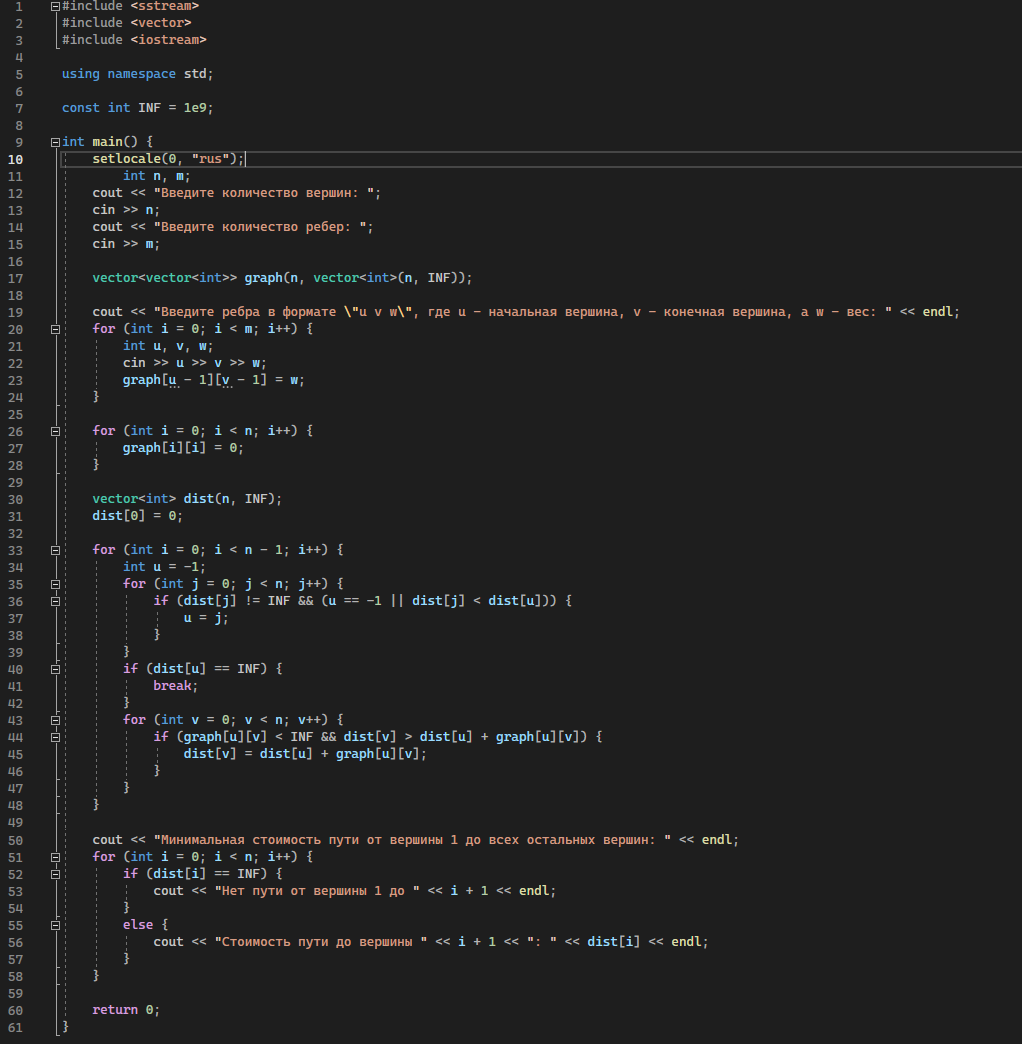
\includegraphics [width=0.9\textwidth]{pelmeni}\\
   
    \label{fig:picResult}
\end{figure}

Код на языке C++ реализует алгоритм Дейкстры для нахождения кратчайшего пути во взвешенном графе с неотрицательными весами ребер. Алгоритм принимает на вход количество вершин и ребер графа, а также информацию о ребрах в формате "начальная вершина, конечная вершина, вес", где вес - это длина ребра.

Сначала мы создаем двумерный массив graph размером n x n и заполняем его бесконечными значениями (INF). Затем вводим ребра и заполняем соответствующие элементы массива graph.

После этого мы обходим все вершины графа и присваиваем диагональным элементам значения 0, т.к. минимальное расстояние до вершины самой себя равно 0.

Далее создаем массив dist размером n и заполняем его бесконечными значениями, кроме первой вершины, до которой минимальное расстояние равно 0.

Затем производим n-1 итераций, выбирая текущую вершину u, имеющую минимальное значение dist и проверяем все смежные с ней вершины v. Если расстояние до v через u является меньшим, чем текущее минимальное расстояние до v, то обновляем значение dist[v].

После выполнения алгоритма выводим на экран минимальную стоимость пути от вершины 1 до всех остальных вершин.

В данном коде также используется vector для хранения двумерного массива graph и одномерного массива dist, что упрощает работу с массивами и позволяет избежать ошибок при использовании динамической памяти.


\begin{figure}[h!]
    \centering
    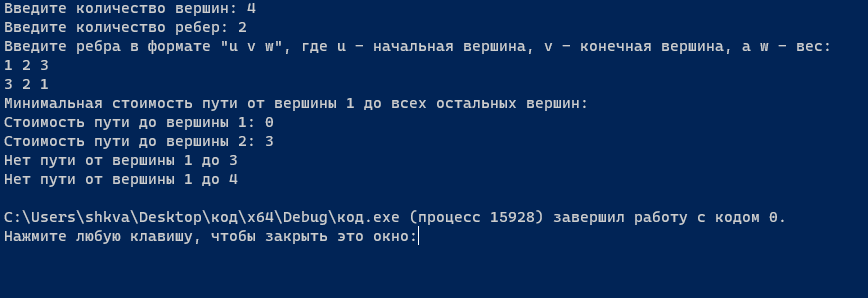
\includegraphics [width=0.9\textwidth]{pelmeni2}\\
    \caption{Результат выполнения программы}
    \label{fig:picResult}
\end{figure}

\newpage \section{Список используемой литературы}

\begin{enumerate}

    \item "Язык программирования C++. Базовый курс" Бьерн Страуструп - Издательство: «Питер», 2006, 1104с.
    \item "Роберт Лафоре. Объектно-ориентированное программирование в С++
    \item "https://www.youtube.com/watch?v=kRcbYLK3OnQ&list=
    
    PLQOaTSbfxUtCrKs0nicOg2npJQYSPGO9r
\end{enumerate}

\end{document}